\chapter{Induction conducteurs immobiles} % (fold)
\label{chap:Induction conducteurs immobiles}

D'après les équations de Maxwell, un champ magnétique dépendant du temps peut engendrer un champ électrique. 

Ce champ électrique est susceptible de mettre en mouvement des charges électriques au sein d'un conducteur et donc de créer des courants. On parle de \textbf{courants induits}.

\section{Conducteur dans un champ magnétique variable} % (fold)
\label{sec:Conducteur dans un champ magnétique variable}

\subsection{Loi d'Ohm locale} % (fold)
\label{sub:Loi d'Ohm locale}

\subsubsection{Modèle de Drude} % (fold)
\label{sec:Modèle de Drude}

Quand on électron se déplace dans un métal, il subit des chocs avec les atomes du temps. Ces collisions freinent le déplacement de l'électron. Il est soumis à une \underline{force de frottement} d'expression : 
\begin{equation}
  \overrightarrow{F_f} = - \frac{m}{\tau} \overrightarrow{v}
  \label{eq:frottement}
\end{equation}
% subsubsection Modèle de Drude (end)

\subsubsection{Analyse dimensionnelle} % (fold)

\begin{equation}
  [\| \overrightarrow{F_f} \|] = \frac{[m]}{[\tau]} [ \| \overrightarrow{v} \|] \implies [\tau] = \frac{[m]}{[F]} [v] = \frac{ML. T ^{-1}}{MLT ^{-2}}  = T
\end{equation}

Remarque : $\tau$ 
\begin{itemize}

    \item représente la \underline{durée moyenne} entre 2 \underline{collisions} 
    \item $\tau$ est appelé \textbf{temp caractéristique d'amortissement}

    \item $\tau \approx 10 ^{-12}$ à $10 ^{-15}$ s

\end{itemize}
% subsubsection Analyse dimensionnelle pour $\tau$ (end)

\subsubsection{Analyse mécanique} % (fold)
\label{sec:Analyse mécanique}

\begin{itemize}

    \item Système étudié : Un électron de charge $q = -e$, de masse $m$ 
    \item Référentiel d'étude : référentiel terrestre supposé galiléen, repère lié au conducteur 
    \item Bilan des forces : 
      \begin{itemize}

          \item Le poids de l'électron : $\overrightarrow{P}$ est négligeable 
          \item La force de frottement \ref{eq:frottement} : $\overrightarrow{F_f} = - \frac{m}{\tau} \overrightarrow{v}$ 
          \item Présence de $(\overrightarrow{E}, \overrightarrow{B})$, force de Lorentz : $\overrightarrow{F_l} = q \overrightarrow{E}+ q \overrightarrow{v} \wedge \overrightarrow{B} \approx q \overrightarrow{E}$

            \begin{myproof}{Raison de négligance}{}
               Or $B = E/c$ dans la vide mais aussi dans le métal, 
               \begin{equation}
                 \frac{qvB}{qE}  = \frac{v}{c}  \ll 1
               \end{equation}
            \end{myproof}

          \item PFD : 
            \begin{gather}
              q \overrightarrow{E} - \frac{m}{\tau} \overrightarrow{v} = m \frac{\mathrm{d}\overrightarrow{v} }{\mathrm{d}t} \text{ or } \overrightarrow{j} = nq \overrightarrow{v} \\ 
              q \overrightarrow{E}- \frac{m}{\tau} \frac{\overrightarrow{j}}{nq} = \frac{m}{nq}  \frac{\mathrm{d} \overrightarrow{j}}{\mathrm{d}t} 
            \end{gather}

      \end{itemize}


          \item En régime statique :  $\frac{\mathrm{d} \overrightarrow{j}}{\mathrm{d} t} = 0$ 
            \begin{gather}
              q \overrightarrow{E} = \frac{m}{\tau} \frac{\overrightarrow{j}}{nq}  \\ 
              \overrightarrow{j} = \frac{n q ^{2}\tau \overrightarrow{E}}{m}  = \gamma \overrightarrow{E}
            \end{gather}

            avec 
            \begin{equation}
              \boxed{\gamma = \frac{n (-e) ^{2}\tau}{m} =\frac{ne ^{2}\tau}{m}}
            \end{equation} 
            est appelé \textbf{conductivité électrique} d'un conducteur. Il dépend du caractéristique du métal ($n$ : densité de charges par unité de volume)

          \item En régime dépendant du temps : 
            \begin{gather}
              q \overrightarrow{E}(t) - \frac{m}{\tau nq}  \overrightarrow{j}(t) = \frac{m}{nq} \frac{\mathrm{d}\overrightarrow{j}(t)}{\mathrm{d}t}  \\ 
              \frac{\mathrm{d} \overrightarrow{j}}{\mathrm{d}t}  (t) + \frac{1}{\tau}  \overrightarrow{j}(t) = \frac{nq ^{2}}{m} \overrightarrow{E}(t) = \frac{\gamma}{\tau}  \overrightarrow{E}
            \end{gather}

          Pour une variation de type sinusoïdale $\underline{\overrightarrow{j}}(t) = j(t) \exp (i \omega t + \varphi _i)$ avec $i ^{2} = -1$.
          \begin{gather}
            \left[i \omega + \frac{1}{\tau} \right] \underline{\overrightarrow{j}} = \frac{\gamma}{\tau}  \underline{\overrightarrow{E}} \\ 
            \underline{\overrightarrow{j}} = \frac{\gamma}{\tau \left(i \omega + \frac{1}{\tau} \right)} \underline{\overrightarrow{E}}  = \left( \frac{\gamma}{1 + i \omega \tau} \right) \underline{\overrightarrow{E}} = \underline{\gamma} \underline{\overrightarrow{E}}
          \end{gather}

          Si $\omega \tau \ll 1$, alors $\overrightarrow{j} = \gamma \overrightarrow{E}$, c'est-à-dire si $f \ll 10 ^{12}$ Hz.
\end{itemize}

\subsection{Charge dans un conducteur ohmique} % (fold)
\label{sub:Charge dans un conducteur ohmique}

\subsubsection{Équation de conservation de la charge et loi d'Ohm locale} % (fold)
\label{sec:Équation de conservation de la charge et loi d'Ohm locale}

\begin{gather}
  \mathrm{div} \overrightarrow{j}(M,t) + \frac{\partial \rho(M,t)}{\partial t}  = 0 \text{ or } \overrightarrow{j}(M,t) = \gamma \overrightarrow{E(M,t)} \\ 
  \mathrm{div} | \gamma \overrightarrow{E}(M,t) | + \frac{\partial \rho(M,t)}{\partial t}  = 0 \text{ or } \text{Maxwell-Gauss} \\ 
  \frac{\partial \rho(M,t)}{\partial t} (M,t) + \frac{\gamma}{\varepsilon_0}  \rho(M,t) = 0
\end{gather}

Hypothèse : À $t=0$ on a créé une densité de charge $\rho_0$. 

\subsubsection{Solutions de l'équation différentielle} % (fold)
\label{sec:Solutions de l'équation différentielle}
 \begin{equation}
   \rho(M,t) = \rho_0 \exp \left( - \frac{\gamma}{\varepsilon_0} t \right) = \rho_0 \exp \left( - \frac{t}{\tau_c}  \right)
 \end{equation}

 avec $\tau_c = \frac{\varepsilon_0}{\tau} $ est appelé \textbf{temps de relaxation des charges}. (ODG : Pour les métaux : $\tau_C \approxeq 10 ^{-19}$ s)

 Conclusion : La charge disparaît presque 
% subsubsection Solutions de l'équation différentielle (end)
% subsubsection Équation de conservation de la charge et loi d'Ohm locale (end)

 \subsubsection{Régime sinusoïdal} % (fold)
 
 % subsubsection subsubsection name (end)
En régime sinusoïdal, de pulsation $\omega$ : 
\begin{gather}
  \frac{\partial \underline{\rho}(M,t)}{\partial t} + \frac{
  \gamma
  }{\varepsilon_0}  \underline{\rho}(M,t) = 0 \\ 
  \left( i \omega + \frac{\gamma}{\varepsilon_0}  \right) \underline{\rho}(M,t) = 0 \implies \underline{\rho} = 0
\end{gather}

En régime sinusoïdal, il est impossible d'établir une densité de charge dans un conducteur.

\subsubsection{Conclusion} % (fold)
\label{sec:Conclusion}

Dans tous les cas, on considère que la densité de charge \underline{dans un conducteur} est nul.
% subsubsection Conclusion (end)

% subsection Charge dans un conducteur ohmique (end)


% subsection Loi d'Ohm locale (end)
% section Conducteur dans un champ magnétique variable (end)

\subsection{Exemple de courant induit} % (fold)
\label{sub:Exemple de courant induit}

\begin{figure}[H] %h:当前位置, t:顶部, b:底部, p:浮动页
  \centering
  \includegraphics[width=0.8\textwidth]{./assets/Solénoïde parcouru par un courant variable.png}
  \caption{Solénoïde parcouru par un courant variable}
\end{figure}


On considère un solénoïde parcouru par un courant variable : 
\begin{equation}
  I(t) = I_0 \cos \omega t
\end{equation}


On obtient : 
\begin{equation}
  \overrightarrow{E}(M,t) = E(r,t) \overrightarrow{e _ \theta}, \; \overrightarrow{B}(M,t) = B(r,t) \overrightarrow{e_z}
\end{equation}

\subsubsection{Condition ARQS magnétique} % (fold)
\label{sec:Condition ARQS magnétique}

% subsubsection Condition ARQS magnétique (end)

Dans l'ARQS magnétique, $I(t)$ varie lentement et $\overrightarrow{B}(M,t) = \overrightarrow{B} _{QS} (M,t)$ : 
\begin{equation}
  \overrightarrow{B}(M,t) = \overrightarrow{B} _{QS}(M,t) = \begin{cases}
    \mu_0 n I(t) \overrightarrow{e_z} \quad (r<R) \\ 
    \overrightarrow{0} \quad (r>R)
  \end{cases}
\end{equation}

\subsubsection{Champ électrique} % (fold)
\label{sec:Champ électrique}

Appliquons la \textbf{loi de Faraday} à un contour fermé circulaire d'axe $Oz$ de rayon $r$ :
\begin{itemize}

    \item Si $r < R$ : 
      \begin{equation}
        \overrightarrow{E}(r < R, t)= - \mu_0 \frac{nr}{2}  I_0 (- \omega) \sin (\omega t) \overrightarrow{e _ \theta}
      \end{equation}

    \item Si $r > R$ : 
      \begin{equation}
        \overrightarrow{E}(r > R, t)= - \mu_0 \frac{nR ^{2}}{2r}  I_0 (- \omega) \sin (\omega t) \overrightarrow{e _ \theta}
      \end{equation}

\end{itemize}
% subsubsection Champ électrique (end)

À l'intérieur du solénoïde, on place un cylindre conducteur de conductivité $\gamma$, de rayon $a$ et de longueur $l$.

% subsection Exemple de courant induit (end)
% chapter Induction conducteurs immobiles (end)


\subsection{Effet de peau} % (fold)
\label{sub:Effet de peau}

% subsection Effet de peau (end)

On se place dans un conducteur ohmique dans lequel existent un champ $\overrightarrow{E}(M,t)$ et un champ $\overrightarrow{B}(M,t)$ dépendant du temps de façon sinusoïdale à la pulsation $\omega$. 

Nous considérons un métal qui occupe le demi-espace $z>0$ : 

Il existe en surface du conducteur un champ magnétique : 
\begin{equation}
  \overrightarrow{B}(z = 0 ^{-}, t) = B_0 \cos (\omega t) \overrightarrow{e_x}
\end{equation}

Dans le conducteur : 
\begin{equation}
  \overrightarrow{E}(z>0, t) = \overrightarrow{E_0} \cos ( \omega t + \varphi_E)
\end{equation}

\begin{figure}[H] %h:当前位置, t:顶部, b:底部, p:浮动页
  \centering
  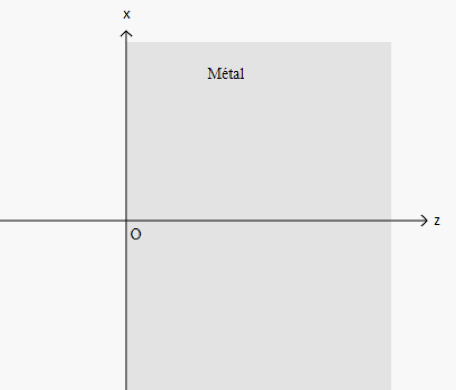
\includegraphics[width=0.5\textwidth]{./assets/Effet de peau.png}
  \caption{Effet de peau}
  \label{fig:Effet de peau}
\end{figure}




\subsubsection{Le courant de déplacement est négligeable devant le courant de conduction} % (fold)
\label{sec:Le courant de déplacement est négligeable devant le courant de conduction}

On les exprime : 
\begin{equation}
  \overrightarrow{j} _{\text{conduction}} = \gamma \overrightarrow{E}  \quad  \overrightarrow{j} _D = \varepsilon_0 \frac{\partial \overrightarrow{E}}{\partial t} 
\end{equation}

Donc, 
\begin{equation}
  \frac{ \| \overrightarrow{j_D} \|}{ \| \overrightarrow{j} \|} = \frac{\varepsilon_0 \omega E_0}{\gamma E_0}  = \frac{\varepsilon_0}{\gamma}  \omega = \omega \tau_c
\end{equation}

avec $\tau_c = \frac{\varepsilon_0}{\gamma} $ temps de relation d'ordre de grandeur $\approx 10 ^{-19}$ s. $\tau_C \ll \tau$

Conclusion : 
\begin{equation}
  \| \overrightarrow{j_D} \| \ll \| \overrightarrow{j} \|
\end{equation}
% subsubsection Le courant de déplacement est négligeable devant le courant de conduction (end)

\subsubsection{Équations de Maxwell modifiées} % (fold)
\label{sec:Équations de Maxwell modifiées}

\begin{gather}
  \mathrm{div} \overrightarrow{E} = 0 \quad (R.S.) \\ 
  \mathrm{div} \overrightarrow{B} = 0 \\
  \overrightarrow{\mathrm{rot}} \overrightarrow{E}= - \frac{\partial \overrightarrow{B}}{\partial t}  \\ 
  \overrightarrow{\mathrm{rot}} \overrightarrow{B} = \mu_0 \overrightarrow{j}
\end{gather}

\subsubsection{Équation de diffusion du type} % (fold)
\label{sec:Équation de diffusion du type}

Pour le champ $\overrightarrow{E}$ : 
\begin{gather}
  \overrightarrow{\mathrm{rot}} (M.F.) \implies \overrightarrow{\mathrm{rot}}(\overrightarrow{\mathrm{rot}} \overrightarrow{E}) = \overrightarrow{\mathrm{rot}} \left( - \frac{\partial \overrightarrow{B}}{\partial t}  \right) = - \frac{\partial }{\partial t} (\overrightarrow{\mathrm{rot}} \overrightarrow{B}) \\
   \overrightarrow{\mathrm{grad}}(\mathrm{div} \overrightarrow{E}) - \Delta \overrightarrow{E} = - \frac{\partial }{\partial t} (\mu_0 \overrightarrow{j} ) = - \frac{\partial }{\partial t} (\Delta \overrightarrow{E}) \mu_0 \\ 
   \boxed{\Delta \overrightarrow{E} = \mu_0 \gamma \frac{\partial \overrightarrow{E}}{\partial t} }
\end{gather}
% subsubsection Équation de diffusion du type (end)

Phénomène \textbf{irréversible} causé par le caractère \underline{dissipatif} de la force de frottement entre les porteurs de charge et le réseau.

Invariance par translation selon $\overrightarrow{e_x}$ et $\overrightarrow{e_y}$ pour le champ $\overrightarrow{B}$. 

\subsubsection{Notation complexe} % (fold)
\label{sec:Notation complexe}

% subsubsection Notation complexe (end)
On peut donc écrire en notation complexe : 
\begin{equation}
  \underline{\overrightarrow{B}}(z,t) = \underline{f}(z) \exp(i \omega t)
\end{equation}
% subsubsection Équations de Maxwell modifiées (end)
